\chapter{Integrating occupancy models and structural equation models to understand species occurrence}
\chapterauthor{Maxwell B. Joseph, Daniel L. Preston, Pieter T. J. Johnson}
\label{ch3}

Understanding the drivers of species occurrence is a fundamental goal in
basic and applied ecology. Occupancy models have emerged as a popular
approach for inferring species occurrence because they account for
problems associated with imperfect detection in field surveys. Current
models, however, are limited because they assume covariates are
independent (i.e., indirect effects do not occur). Here, we combined
structural equation and occupancy models to investigate complex
influences on species occurrence while accounting for imperfect
detection. These two methods are inherently compatible because they both
provide means to make inference on latent or unobserved quantities based
on observed data. Our models evaluated the direct and indirect roles of
cattle~grazing, water chemistry, vegetation, nonnative fishes, and pond
permanence on the occurrence of six pond-breeding amphibians, two of
which are threatened: the California tiger salamander (\textit{Ambystoma
californiense}), and the California red-legged frog (\textit{Rana
draytonii}). While cattle had strong effects on pond vegetation and
water chemistry, their overall effects on amphibian occurrence were
small compared to the consistently negative effects of nonnative fish.
Fish strongly reduced occurrence probabilities for four of five native
amphibians, including both species of conservation concern. These
results could help to identify drivers of amphibian declines and to
prioritize strategies for amphibian conservation. More generally, this
approach facilitates a more mechanistic representation of ideas about
the causes of species distributions in space and time. As shown here,
occupancy modeling and structural equation modeling are readily
combined, and bring rich sets of techniques that may provide unique
theoretical and applied insights into basic ecological questions.~

\section{Introduction}

Much of ecology is concerned with explaining and predicting where
species occur in space and time. While species distributions are
directly and indirectly influenced by a diverse suite of abiotic and
biotic factors, most statistical treatments do not formally
differentiate between direct and indirect effects \citep{Guisan2005}. Structural equation modeling (SEM) provides one means by which to
formally represent causal assumptions in the form of direct and indirect
causal pathways, helping to close the gap between biological mechanisms
and statistical methodology \citep{Bollen1989, Grace2006}.

Structural equation models combine causal assumptions with observations
to generate causal inferences \citep{Pearl2000}. Often, these assumptions are
displayed in a path diagram that represents model components and causal
relationships (i.e.~how one variable affects another). These path
diagrams encode both direct and indirect effects, such as those involved
in complex processes that structure communities \citep{clough2012, Alsterberg2013}.
As a result, SEM provides a framework for clarifying,
representing, and evaluating hypotheses in ecology that can outperform
traditional associational statistical methods. For example, the
relationship between productivity and biodiversity has historically been
evaluated statistically in a bivariate context, despite the
multidimensionality of the hypotheses that have been put forward to
explain the relationship. By explicitly representing causal
relationships between productivity and diversity, along with disturbance
and stressors in a SEM, the mechanistic relationship between
productivity and biodiversity becomes more clear, with more predictive
power than bivariate approaches \citep{Grace2014}. In addition, SEM is
flexible, with recent developments facilitating non-linear effects and a
wide range of distributions, broadening the potential applicability of
SEM in ecology \citep{Lee2007b}. Finally, SEM differentiates between latent
and observable variables. Latent variables cannot be observed directly,
but observations can provide information on latent quantities. A classic
example is the presence or absence of a species.

In practice, studies of species occurrence are notoriously plagued by
imperfect detection because species may be present but unobserved. This
can be problematic when trying to explain species distributions because
false absences create bias in estimated coefficients for covariates that
explain occurrence. For instance, if turbidity increases the probability
of occurrence of an aquatic organism, but decreases detectability
(i.e.~the organism is harder to observe), detection events will not
appear to be related to turbidity. However, adjusting for imperfect
detection facilitates unbiased estimation of the true relationship
between such a factor and species occurrence. Such adjustments can be
made via occupancy modeling, a method in which repeat surveys are used
to estimate probabilities of detection and draw inferences on true
occupancy states \citep{MacKenzie2002}. Occupancy models are classic
hierarchical models, where the latent binary occurrence state is partly
observed, and the extra zeros in detection histories are modeled as
potentially arising from a combination of true and false absences. As
the appreciation and application of occupancy models has increased, they
have been extended to include multiple species, temporal dynamics
including colonization and extinction, estimation of species richness,
habitat ephemerality, and even disease dynamics \citep{Dorazio2010, MacKenzie2011, Miller2012}.
These developments have been
instrumental in improving inferences about the processes that govern
species distributions. However, many existing models require independent
covariates for occurrence and detection. This limitation represents a
challenge to understanding even moderately complex processes that drive
species distributions that may include a combination of direct and
indirect effects on occurrence and detectability.

Here, we show that combining SEM with occupancy models overcomes this
limitation and provides a means by which to more directly represent
processes that influence species occurrence. We aim to illustrate the
practical and conceptual compatibility of occupancy modeling and
structural equation modeling by developing a causal model of species
occurrence and community composition that explicitly accounts for
non-detection. We use pond-breeding amphibians as an applied case
example. First, we outline the logic behind the model by summarizing the
relevant empirical knowledge for our system in terms of the effects of
pond permanence, cattle grazing, nonnative fishes, water chemistry, and
vegetation on amphibian occurrence. We then discuss the data collection
scheme and formally relate our observations to the processes under
consideration by developing observation, process, and parameter (prior)
models. As a model verification step, we demonstrate the recovery of
parameters from our SEM using simulation \citep{Rykiel1996}. Last, we present
results for the case study and discuss the value, limitations, and
future directions for this approach.

\section{Study system}

The amphibian community in freshwater ponds of the San Francisco Bay
Area of California, USA includes the Pacific chorus frog
(\textit{Pseudacris regilla}), western toad (\textit{Anaxyrus boreas}),
California newt (\textit{Taricha torosa}), California tiger salamander
(\textit{Ambystoma cailforniense}), California red-legged frog (\textit{Rana
draytonii}), and nonnative American bullfrog (\textit{Lithobates
catesbeianus}) \citep{stebbins2003}. Of the native species, two are federally
protected and are of broad conservation concern (\textit{A. californiense}
and \textit{R. draytonii}), and \textit{A. boreas} has declined in specific
regions \citep{lannoo2005}. Some populations of these species are currently
threatened by invasive species including nonnative fishes and bullfrogs,
which potentially act as predators and competitors for native amphibians
\citep{Fisher1996, lawler1999, Preston2012}.
Further, widespread cattle grazing in this region has the potential to
affect the population dynamics of amphibians at breeding sites directly
via trampling, and indirectly by removing vegetation and increasing the
concentration of nitrogenous compounds in wetlands \citep{Robins2002, Roche2012}.
The ponds we considered included both
temporary and permanent water bodies up to 7 meters in depth.

\section{Data collection}

From 2009 to 2013, field crews used standardized methods to assess
amphibian site occupancy in 171 wetlands in the San Francisco Bay Area,
USA (Contra Costa, Alameda, Santa Clara, and San Mateo counties) \citep{Johnson2013}.
For simplicity, we used only one year of data
from each site (with years chosen at random). The sites consisted of
both artificially created livestock ponds and natural wetlands. Crews
surveyed wetlands twice per summer using a combination of visual
encounter, seine, and dipnet surveys \citep{Crump1994}. Visual
encounter surveys involved a single observer walking the perimeter of
the wetland and recording all species observed. Dipnet sweeps were
conducted every 3 m around the pond perimeter (1.4 mm mesh and 2600
cm$^2$ net area) and three to four seine net hauls were performed in the
deepest regions of each pond (4 mm mesh size and 1 x 2 m net area). For
each survey, we recorded all life stages of each observed amphibian
species. We considered sites ``occupied'' if larval amphibians were
present, which indicates adult presence, successful fertilization, some
degree of larval development, and potential for metamorphosis
(i.e.~breeding activity).

We quantified cattle grazing intensity, percentage of shoreline
vegetated, pond permanence, water chemistry, and the presence of
nonnative fish. To measure cattle grazing intensity, we recorded the
number of cow paddies within three meters of shoreline and recorded
shoreline perimeter with a handheld GPS unit to quantify cow paddy
density at each pond. As a second measure of grazing intensity, we made
a qualitative judgment of whether the wetland was disturbed by cattle
based on evidence of tracks and trampling. Water samples were collected
in acid-washed Nalgene bottles, filtered, frozen, and analyzed for
ammonium (NH$4^+$) and total dissolved nitrogen (TDN) concentrations
using standard protocols (see:
http://snobear.colorado.edu/Kiowa/Kiowaref/procedure.html). Imagery from
Google Earth was used to help determine whether wetlands were permanent,
based on consistent presence of water year round. Last, crews estimated
the percentage of pond shoreline that was vegetated and recorded whether
fish were present or absent using observations from all sampling
methods. The most common fish species were nonnative, including
mosquitofish (\textit{Gambusia affinis}), largemouth bass
(\textit{Micropterus salmoides}), and bluegill sunfish (\textit{Lepomis
macrochirus}).

\section{Conceptual model}

Drawing upon previous literature, we developed a multivariate hypothesis
about the drivers of amphibian community composition in this system
(Figure \ref{3-1}). We expected fish to strongly affect community composition,
particularly species with poor avoidance strategies and high
palatability \citep{Kruse1984, Kats1988, Adams2000, Welsh2006b}.
Further, pond permanence should increase bullfrog
occurrence because bullfrogs have a multi-year larval development period
that is longer than most western native species \citep{Collins1979}. We
hypothesized that livestock would physically alter wetland ecosystems
via trampling and grazing, and chemically alter wetlands via inputs of
nitrogenous waste products in urine and feces \citep{adams2009, Schmutzer2008, Jansen2003207, Knutson2004, Kauffman1983}.
Previous studies indicate that characteristics of
shoreline vegetation influence amphibian breeding and that water
chemistry can alter reproductive success and occupancy probability \citep{Earl2009, Burne2005, Egan2004, Jansen2003207, Brodman2003, Rouse1999, rowe1995, freda1986}.
Separating out the causal
pathways through which grazing alters amphibian occupancy is important
from a practical standpoint, as each one might be targeted differently
with management interventions (e.g., limiting cattle-induced damage to
vegetation versus limiting the total intensity of grazing).

\section{Model formalization}

To formalize the model of Figure \ref{3-1}, we adopted a hierarchical Bayesian
approach, developing model components related to observations, processes
in the system, and priors for unknown parameters \citep{Lee2007b, Cressie2009, Dorazio2010}.

\subsubsection{Observation model}

While early structural equation models assumed normally distributed
observed indicator variables, current methods are extremely flexible in
terms of likelihood functions and relationships between variables,
broadening the applicability of these methods in ecology \citep{Grace2006, Lee2007b}.
We consider the presence/absence state of a species at a
location to be a hidden (latent) binary variable which gives rise to
imperfect detection/nondetection data. The use of a latent state
variable is a key conceptual link between the fields of SEM and
occupancy modeling. The flexibility of this approach is demonstrated in
the following sections where we apply a variety of observation models
from the exponential family, a moderately complex finite-mixture
distribution, and a combination of continuous and discrete latent
variables.

We considered grazing intensity by cattle to be a continuous latent
quantity that cannot be observed directly, whose value is indicated by
evidence of disturbance and the density of cow paddies in the vicinity
of a wetland. Specifically, cattle disturbance was modeled as a
Bernoulli random variable with latent grazing intensity ($\xi$) as a
continuous covariate:

\[ Y_1[j, k] \sim Bernoulli(p_{Y_1}[j]) \]
\[ logit(p_{Y_1}[j]) = \beta_{Y_1, 0} + \beta_{Y_1, 1} \xi[j] \]

for the $j^{th}$ site and the $k^{th}$ survey, with square brackets
representing indexing. Observed cow paddy counts are treated as a second
indicator (specifically, a multi-method indicator) \citep{Grace2006} and
modeled as a Poisson random variable with an offset for shoreline
perimeter of site $j$ ($\mu_{perim}[j]$) in meters:

\[ Y_2[j, k] \sim Poisson(\lambda[j, k]) \]
\[ \dfrac{\lambda_{j, k}}{\mu_{perim}[j, k]} = e^{\beta_{Y_2, 0} + \beta_{Y_2, 1} \xi[j]} \]

Perimeter observations are subject to measurement error and variation
within a season. Therefore, we modeled latent mean perimeter values for
each site ($\mu_{perim}$), which represents the expected pond perimeter
value for site $j$:

\[ log(perim[j, k]) \sim N(\mu_{perim}[j], \sigma_{w}) \]
\[ \mu_{perim}[j] \sim N(\alpha_{perim}, \sigma_{a}) \]

where $\sigma_{w}$ represents measurement error and variation within a
season, $\alpha_{perim}$ is the (log) average perimeter across all
wetlands, and $\sigma_{a}$ is the variability in perimeter among
wetlands.

Shoreline vegetation, $v$, ranged from 0-100\% with a non-negligble
number of 0\%, 100\%, and intermediate observations. Therefore, we
treated these observations as arising from a zero-one inflated beta
distribution, which is a finite mixture distribution with a Bernoulli
component that produces 0's and 1's, and a beta component that produces
values on the interval $(0, 1)$ \citep{Ospina2012}:

\[
P(v; \alpha, \mu_{v}, \phi) = \left\{
  \begin{array}{lr}
    \alpha(1 - \mu_{v}) &  v = 0\\
    \alpha \mu_{v} &  v = 1\\
    (1 - \alpha)f(v; \mu_{v}, \phi) &  0 < v < 1
  \end{array}
\right.
\]

\[ logit(\mu_{v}[j]) = \beta_{v, 0} + \beta_{v, 1} \eta_1[j] \]

\[ logit(\alpha) = a_0 + a_2 \mu_v^2 \]

Here, $\alpha$ determines the extent to which the beta or binomial
mixture components dominate the probability density function. The second
degree polynomial term with coefficient $a_2$ causes extreme values of
the logit-expected shoreline vegetation cover $\mu_v$ to increase the
probability of an observer recording either 0\% or 100\% shoreline
vegetation cover. This formulation essentially imposes a minimum
probability of observers recording a discrete value when the true
shoreline vegetation is 50\%, and increases the probability of 0\% or
100\% observations as the true cover approaches those values. Last,
$f(v; \mu_{v}, \phi)$ is the probability density function of the beta
distribution, parameterized in terms of its mean ($\mu_v$) and variance
($\phi$), which represents the combination of observation error and
within-summer variation in true shoreline vegetation cover \citep{Ospina2012}.

Log-transformed concentrations of ammonium and total dissolved N in the
water were used as multi-method indicators of latent N concentration.
Because both total dissolved N and $NH_4^+$ concentrations tend to
increase over the course of the summer due to exogenous inputs and pond
drying, we also included an effect of survey number $k$, coded as an
indicator variable for the 2nd survey, such that $I(k=2)=1$, and
$I(k=1)=0$.

\[ log(NH_4^+[j, k]) \sim N(\beta_{NH_4^+, 0} + \beta_{NH_4^+, 1} \eta_2[j] + \beta_{NH_4^+, 2} I(k), \sigma_{NH_4^+}) \]

\[ log(N[j, k]) \sim N(\beta_{N, 0} + \beta_{N, 1} \eta_2[j] + \beta_{N, 2} I(k), \sigma_N) \]

We adopt an occupancy modeling approach for the data model describing
amphibian detection and non-detection. Observations of the $i^{th}$
species at the $j^{th}$ site on the $k^{th}$ repeat survey are
represented by $Y[i, j, k]$. We treated these observations as Bernoulli
random variables with probability $p[i, j, k] z[i, j]$, where $p$ is the
probability of detection and $z$ is the latent binary presence/absence
state. The true occurrence state $z$ is only partly observed. If species
$i$ was seen at site $j$ on any survey, it was present, but if it was
not seen on any survey, it is possible that it was present but
unobserved \citep{MacKenzie2002}:

\[ Y[i, j, k] \sim Bernoulli(p[i, j, k] z[i, j]) \]

We treated fish presence and pond permanence as directly observed
quantities, which is supported by consistency of observations within and
across years in this system.

\subsubsection{Process model}\label{process-model}

Our process model represents the latent processes connecting the latent
quantities: grazing intensity $\xi$, shoreline vegetation $\eta_1$, N
concentration $\eta_2$, the true occupancy states $z$, and the
probability of detection $P$ (Figure \ref{3-2}). In the SEM lexicon, process
models are sometimes referred to as structural models. Note that there
is an additional pathway from fish to nitrogen that was not initially
hypothesized, but revealed in the process of model evaluation (see Model
Assessment below).

We treat grazing intensity as an exogenous latent variable, unaffected
by the other latent quantities, with mean $0$ and standard deviation $1$
as an identifiability constraint. Due to cattle grazing on and trampling
of shoreline vegetation, we modeled a linear effect of cattle grazing
intensity $\xi$ on shoreline vegetation $\eta_1$:

\[\eta_1 \sim N(\gamma_{1} \xi, 1)\]

where the standard deviation term, similarly set to 1 for
identifiability, represents the influence of other, unmodeled factors on
shoreline vegetation cover. Nitrogenous inputs from cattle excretion in
and around wetlands are treated similarly. Following a graphical check
of independence assertions, we included an effect of fish presence
($\gamma_3$) on nitrogen:

\[\eta_2 \sim N(\gamma_{2} \xi + \gamma_3 fish, 1).\]

We represented true occupancy states as Bernoulli random variables with
probability of occupancy $\psi[i, j]$ for the $i^{th}$ species at the
$j^{th}$ site, such that $z[i, j] \sim Bernoulli(\psi[i,j])$. We use a
logit-link to model the effects of observed and latent covariates on
$\psi$:

\[ logit(\psi[i, j]) = \alpha_{species}[i] + \alpha_{region}[i, r[j]] + \alpha_{site}[i, j]\]

where $\alpha_{species}$ accounts for species-specific differences in
overall occupancy across the entire study area, $\alpha_{region}$
accounts for regional differences in occupancy rates within each species
(with region $r$ being indexed by site $j$). Last, $\alpha_{site}$
represents the local effects of fish, pond permanence, grazing,
shoreline vegetation and nitrogen concentrations. These terms can be
decomposed as follows:

\[\alpha_{region}[i, j] \sim N(0, \sigma_{\alpha_{region}}[i])\]

This varying intercept term accounts for among-region variation within
species in occupancy, with varying species-specific standard deviations,
to account for the fact that the degree of regional variation in
occupancy rates varies among species. Local covariate effects enter the
final term:

\[\alpha_{site}[i, j] = \beta_{\psi}[i, 1] fish[j] + \beta_{\psi}[i, 2] perm[j] + \beta_{\psi}[i, 3] \eta_1[j] + \beta_{\psi}[i, 4] \eta_2[j] + \beta_{\psi}[i, 5] \xi[j]\]

Species vary in their detection probabilities and $p$ may also vary
between first and second visits:

\[ logit(p[i, j, k]) = \alpha_{p}[i] + \beta_{p} k \]

where $\alpha_{p}$ is a species-specific mean and the last term
represents the effect of early vs.~late summer surveys.

\subsubsection{Priors}

We assumed logit-normal species responses to covariates with
covariate-specific community means and variance parameters that
represent among-species variability, such that:

\[ \beta_{\psi} \sim N(\mu_{\beta_{\psi}}, \sigma_{\beta_{\psi}}) \]
\[ \beta_{p} \sim N(\mu_{\beta_{p}}, \sigma_{\beta_{p}}) \]

Further, we assumed that for each species, mean detection probabilities
would be logit-normally distributed around community level means:

\[ \alpha_{p} \sim N(\mu_{\alpha_{p}}, \sigma_{\alpha_{p}}) \]

Hierarchical parameters corresponding to community-level variance terms
received semi-informative half-Cauchy priors that were weighted towards
small values to reduce bias relative to commonly used uniform priors
\citep{gelman2006}. We adopt vague priors for all other parameters except the
loading terms for indicator variables which were constrained to be
positive (e.g., increases in latent grazing intensity $\xi$ correspond
to increases in its indicators $Y_1$ and $Y_2$). Last, prior information
based on previous work has entered the model in the form of included
effect pathways (e.g., we assume that amphibian community composition
does not affect grazing intensity).

\section{Estimation}

We used \href{http://mc-stan.org/}{Stan}, and the R package
\href{http://mc-stan.org/rstan.html}{rstan} to draw samples from the
joint posterior distribution of all parameters \citep{stan-manual:2014, R2014, rstan-software:2014, stan-software:2014}.
Although this model could be
implemented with WinBUGS, OpenBUGS, or JAGS, the simultaneous updating
of all parameters via the No-U-Turn sampler in Stan results in faster
convergence and more efficient sampling \citep{Hoffman2014}.
Running three chains in parallel with 30000 iterations took about 80
minutes on a quad-core i7 laptop. Convergence was assessed using visual
inspections of trace plots and the Gelman-Rubin potential scale
reduction factor \citep{Gelman1992, Brooks1998}.

\section{Model assessment}

As this is a new method, we conducted a simulation analysis to ensure
adequate recovery of parameter estimates across a range of known values.
We simulated approximately 100 datasets with structure identical to our
model, and the same amount of information (observations) present in our
dataset. We then attempted to recover the known parameters by fitting
the model to our simulated datasets \citep{Gimenez2012}. Any
simulations that did not reach convergence at the MCMC step were
discarded.

Independence assumptions were evaluated graphically using scatter plots
to detect missing causal pathways \citep{Grace2012}. This revealed a
positive correlation between fish presence and N (both total dissolved N
and $NH_4^+$), leading to the inclusion of an additional effect of fish
on N that we had not initially hypothesized. Mechanistically, this
pathway may represent the joint effects of fish locking up N in their
tissues, and suppressing zooplankton through predation, leading to
release of phytoplankton from grazing and greater uptake of N from the
water \citep{Andersson1978, Henrikson1980}.

\section{Results}

\subsection{Parameter recovery}

Our simulations demonstrated parameter recovery with 95\% highest
density posterior intervals (HDIs) including the true population level
parameters over 90\% of the time (Figure \ref{3-a1}). Furthermore, we were able
to recover effects of local factors ($\beta_\psi$), identifying large
effects as being non-zero (Figure \ref{3-a2}). These results increased
confidence in parameter estimates for the empirical data and gave an
indication of the power that we might have to detect effects of local
drivers of occurrence with a dataset of comparable size.

\subsection{Empirical results}

Nonnative fish and pond permanence directly affected amphibian community
composition, with fish exerting the most consistent and strongest
effects. Nonnative fish reduced the probability of occurrence for four
of five native amphibians (all species except western toads and
bullfrogs; Figure \ref{3-3}). Species-specific effects were observed for pond
permanence, which had a strong positive effect on bullfrog and
red-legged frog occurrence. Shoreline vegetation, nitrogenous compounds,
and cattle grazing exerted relatively weak direct effects, with all HDIs
including zero. Similarly, all HDIs for indirect effects of fish (via
nitrogen) and cattle (via nitrogen and shoreline vegetation) on
amphibian occurrence included zero.

Consistent with our expectations and previous work, cattle grazing
decreased shoreline vegetation (HDI: (-0.556, -0.206)) and increased
nitrogenous compounds in the water column (HDI: (0.097, 0.450)). The
grazing submodel combined information from cow paddy density counts and
disturbance classifications to generate values of latent grazing
intensity for each site (Figure \ref{3-4}). As we expected based on field
observations, many sites experience moderate to high levels of grazing,
while fewer experience very low levels of grazing.

Regionally, some species were far more variable in their distribution
among parks than others. For example, although local factors tended to
have minimal effects on the distribution of western toads (Figure \ref{3-3}),
among-region variability was quite high for this species (Figure \ref{3-a3}). In
contrast, Pacific chorus frogs had low among-park variability, being
nearly ubiquitous.

Most amphibian species were easier to detect during the first survey,
probably due to metamorphosis occurring before or during the late-summer
visit when evidence of successful breeding is no longer detectable
(Figure \ref{3-a4}). The inclusion of the visit number covariate (first
vs.~second) accounted for this discrepancy in the sense that
species-specific covariate effects can still be recovered (Figure \ref{3-a2}).

The shoreline vegetation submodel performed well, capturing the fact
that some shorelines were either devoid or completely covered by
vegetation, with variability between these two extremes (Figure \ref{3-4}). The
latent N variable and observed log-transformed total dissolved N and
$NH_4^+$ concentrations showed good fit, with increasing N
concentrations in late summer compared to early summer (Figure \ref{3-4}).
Graphical checks of independence assertions indicated no further causal
pathways for inclusion (Figure \ref{3-a5}).

\section{Discussion}

Our approach demonstrates the integration of SEM with occupancy modeling
using a large-scale survey of pond breeding amphibians to gain a better
understanding of the drivers of community composition. Importantly, this
approach allows for explicit differentiation between observed data and
underlying processes, accounting for a variety of measurement error
models including the imperfect measurement process that gives rise to
species detection data. We also embedded other types of observation
models to account for more complicated likelihood functions, including
the zero-one inflated beta distribution that was used to model
observations of shoreline vegetation cover. With this approach, latent
ecological processes hypothesized to drive occurrence can be explicitly
represented and their direct and indirect consequences formally
evaluated.

The potential advantages of integrating occupancy and structural
equation frameworks include: 1) developing more mechanistic approaches
for understanding species distributions influenced by simultaneous
related processes; 2) inheriting a formal method for evaluating
potential outcomes that would result from management interventions; and
3) clarifying hypotheses by requiring that assumptions be represented in
a formal causal model. Unlike purely associational methods, the causal
assumptions embedded within structural equation models facilitate unique
predictions that can be used to answer applied management questions.

Well-specified SEMs yield unique management insights based on ``do''
operators, which can estimate the consequences of targeted interventions
from effect decompositions \citep{PEARL1998}. ``Do'' operators could be used
to predict changes in occupancy following a management intervention that
reduces grazing intensity or removes fish. Indeed, this was one of the
original arguments for the development of structural equation models in
the mid-20th century \citep{shipley2002cause}. Causal inferences
drawn from such analyses can be no better than the validity of the
assumptions used to construct the model, however. Processes that drive
the species distributions can be represented best when there is
substantive knowledge to construct such models. This brings up two
issues: how mechanistic is ``mechanistic enough'', and how valid are the
assumed causal relationships? First, it would be unreasonable to expect
to construct an infinitely accurate and specific causal model for the
occurrence of any species \citep{shipley2002cause}. However, an adequate model may
capture the most important drivers of occurrence and provide
``good-enough'' predictions for management interventions. This point
underlines the role of interventional tests of such models - if the true
outcome of management intervention deviates from anticipated effects,
then the validity of the underlying causal model must be questioned.

Although not a substitute for interventions, tests of model fit to
observational data can also be useful for identifying potentially
missing pathways based on independence relationships among variables in
the causal network. Here, we employed graphical checks of independence
assumptions for observed variables, but better methods could be
developed. Information theoretic and d-separation tests exist for path
analytic models, and other indices of model fit have long been used for
traditional linear structural equation models that assume multivariate
normality of errors \citep{Grace2006, Shipley2013}. However, methods for
evaluating occupancy model fit are still relatively new and mostly rely
on out-of-sample data \citep{Zipkin2012} or bootstrapping \citep{MacKenzie2004}. Developing methods to evaluate the fit of hierarchical
occupancy-type structural equation models with non-normal indicators and
binary, partially observed latent variables is a non-trivial task, but
one that would increase the utility of this method. Advances in the
study of probabilistic graphical models may provide solutions, but such
advances are only just beginning to be applied by ecologists \citep{Koller2009, Grace2012}.
Aside from d-separation tests,
management experiments provide another way to test the predictive power
of these types of models.

\section{Management implications}

Our results have direct relevance to the management of threatened
amphibian populations within lowland wetlands in California,
particularly when land managers are faced with multiple potential
challenges simultaneously. Livestock grazing, which is common throughout
the western United States \citep{fleischner1994}, has been a topic of
uncertainty with regard to amphibian conservation. While several studies
indicate negative overall effects of grazing on populations of specific
amphibian species \citep{Knutson2004, Schmutzer2008}, others
indicate the potential for positive effects of grazing on diversity and
the perseverance of native communities \citep{Marty2005}.

Based on our analysis, livestock grazing in the Bay Area of California
had minimal effects on the occurrence of six amphibian species, two of
which are native species of conservation concern. This finding suggests
that current grazing levels employed on these parks may be compatible
with management aimed at conserving threatened amphibians. However, we
did not explore the effects of grazing on amphibian abundance or
temporal dynamics such as persistence and colonization. Such approaches
may reveal effects of grazing that were not seen in this study.

Most ponds in this data set were initially constructed to serve as
watering sites for livestock. Because most original natural wetlands in
California have been destroyed for agriculture and development,
particularly in the Central Valley \citep{Garone2011}, such livestock ponds
may now serve as vital habitat refuges for declining species. This trend
is particularly important for the California tiger salamander and
California red-legged frog, which are the focus of considerable
conservation efforts due largely to habitat destruction \citep{lannoo2005}.

In sharp contrast to the minimal effects of grazing, we found strong
negative effects of nonnative fish on native amphibian occupancy for all
species except western toads and nonnative bullfrogs. This finding
supports a large body of research showing that native pond-breeding
amphibians that lack evolutionary history with fishes are unlikely to
persist once predatory fish have been introduced to a breeding site. The
most common fish species at our field sites were mosquitofish and
centrarchids (bass, bluegill and other sunfish), which are native to the
eastern United States. These species likely prevent amphibian
reproduction through direct predation on multiple life stages of native
amphibians. The lack of an effect on toads is consistent with prior work
showing that toxicity and schooling behavior of toad larvae provides
resistance to predation by fish \citep{Kruse1984, Welsh2006b}.
Bullfrogs, which require permanent water bodies to complete
metamorphosis, have co-evolved with fish in their native range, are
unpalatable, and are not strongly affected by fish presence \citep{walters1975, Kruse1977, Szuroczki2011}.

Taken together, our results indicate that land management strategies
should prioritize removal of nonnative fish rather than limitation of
livestock grazing. Fish removal via pond draining has been shown to be
effective in restoring populations of threatened amphibians within the
study region \citep{Alvarez2003}. Considering the needs of interests
groups involved and the prevalence of grazing, this strategy is perhaps
more feasible than dramatically limiting access of livestock to ponds,
which may have unintended side effects including elimination of pond
breeding habitat due to overgrowth by vegetation. While more research is
needed to evaluate both temporal effects of grazing, and how grazing
affects amphibian abundance, our analysis indicates that fish
introductions have more severe impacts than cattle grazing.

\subsection{Conclusion}

Structural equation modeling provides a framework to evaluate why
species occur in some areas and not others, allowing a more direct
confrontation of some of the most fundamental questions in ecology.
Occupancy modeling provides a solution to the problem of imperfect
detection and can account for many different processes giving rise to
detection data. Combining these approaches provides a means to evaluate
complex causal processes driving occurrence while accounting for
false-absences in empirical occurrence data. This framework potentially
facilitates deeper insights into biological processes, making a clear
separation between imperfectly observed data and underlying states. From
a pragmatic standpoint, it is clearly advantageous to be able to
represent both direct and indirect determinants of species occurrence
rather than being limited to treating covariates as being independent.
This approach also provides the practical advantage of inheriting a
suite of methods to anticipate the effects of management interventions
(``do'' operators), and to account for many different sampling schemes
in the occupancy modeling literature. Future extensions of this method
could deepen connections between SEM and other classes of occupancy
models, including dynamic multi-year occupancy models, models of
abundance such as N-mixture models, Dail-Madsen models, their
multi-species extensions, and spatial models \citep{Royle2004, Royle2007, Dail2011, Lamb2014, Dorazio2014}.

The full value of this approach may be most apparent, and perhaps
palatable to individuals unfamiliar with SEM, when coupled with
controlled field experiments, where the validity of the underlying
causal model may be tested directly. Compared to fields like sociology
and economics, ecology as a field is perhaps in a unique position to
reap benefits from SEM because it is both complex and relatively
amenable to experimental manipulation.

\begin{figure}[htbp]
\caption[Conceptual model showing influences on amphibian breeding success.]{
Conceptual model showing influences on amphibian breeding success. Nodes
represent concepts of interest, and directional arrows represent causal
effects (e.g.~grazing intensity affects shoreline vegetation)
}
\centering
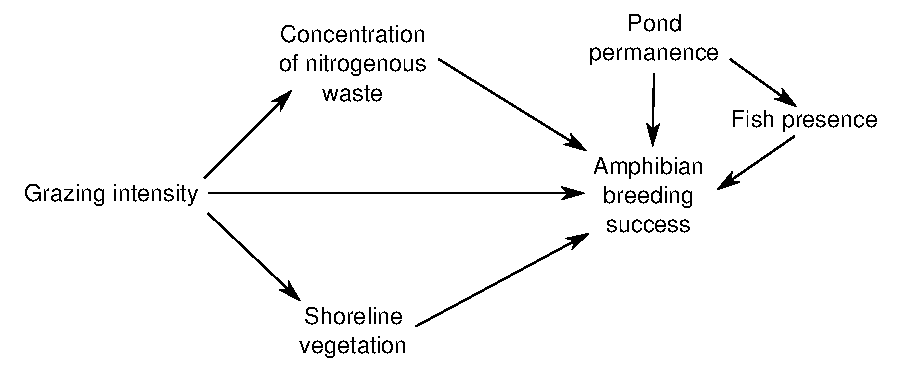
\includegraphics[width=150mm]{figs/ch3/fig1.pdf}
\label{3-1}
\end{figure}

\begin{figure}[htbp]
\caption[DAG relating latent and observed variables.]{
Directed acyclic graph illustrating relationships between unknown
quantities (circles) and observed indicator variables (rectangles).
}
\centering
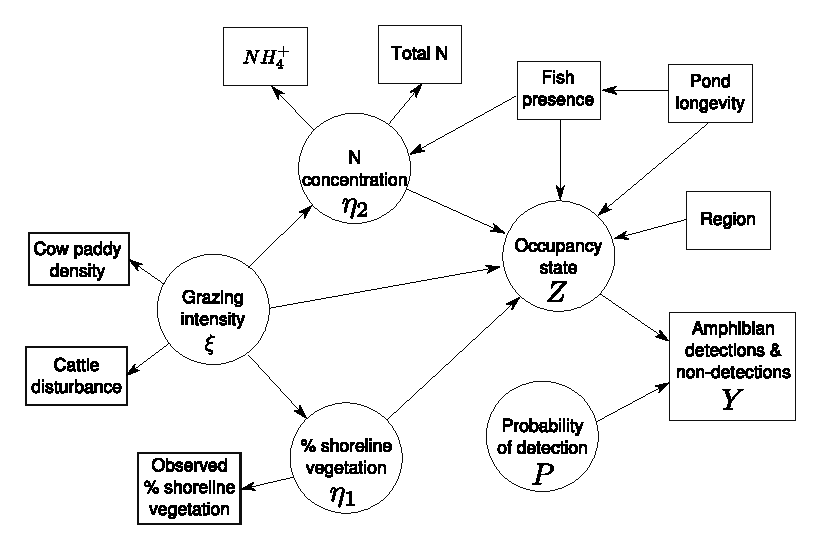
\includegraphics[width=150mm]{figs/ch3/fig2.pdf}
\label{3-2}
\end{figure}

\begin{figure}[htbp]
\caption[Direct effects on amphibian occurrence]{
Estimated direct effects on occurrence probabilities for each species.
Black corresponds to parameters for which HDIs excluded zero, and grey
correpsonds to HDIs including zero
}
\centering
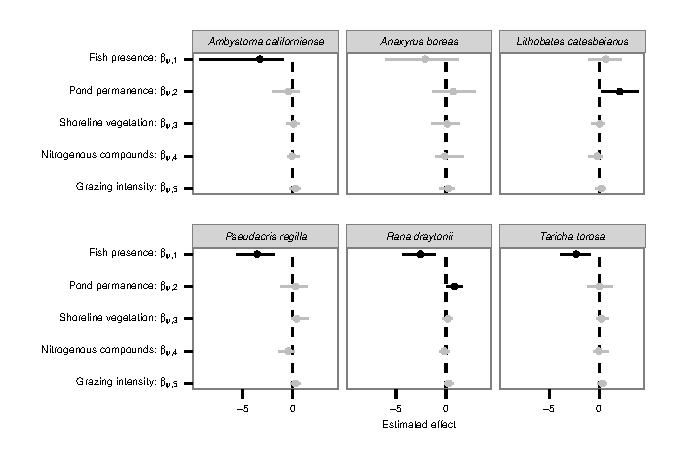
\includegraphics[width=150mm]{figs/ch3/fig3.pdf}
\label{3-3}
\end{figure}

\begin{figure}[htbp]
\caption[Submodel fit for observed indicator variables]{
Fit of the submodels to the observed indicator variables. Shaded regions
encompass the 95\% HDI, with observed data shown as jittered points
(x-axis values represent posterior medians).
}
\centering
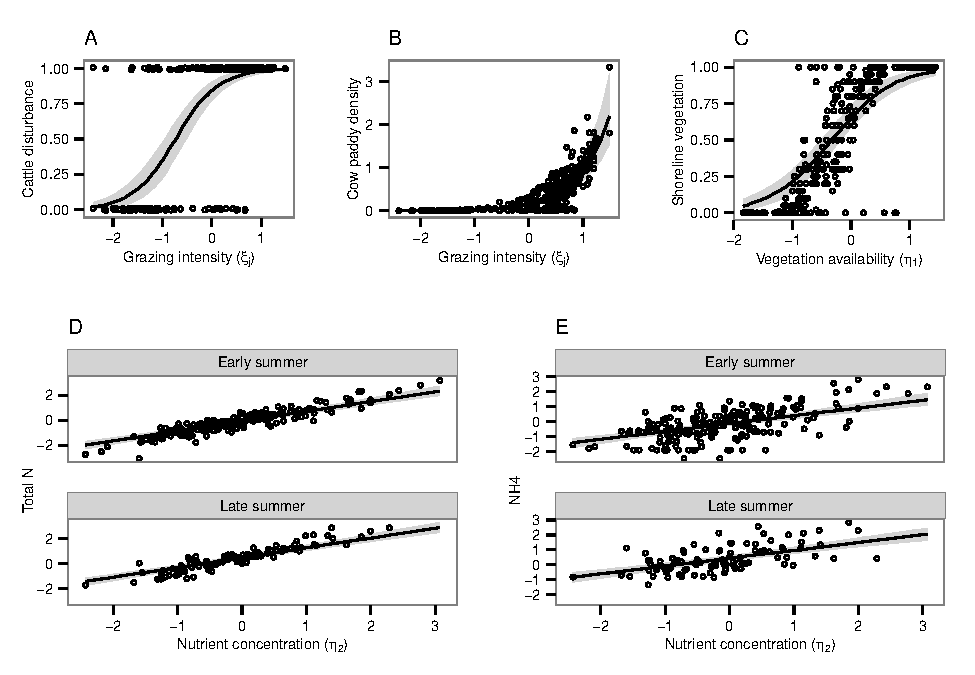
\includegraphics[width=150mm]{figs/ch3/fig4.pdf}
\label{3-4}
\end{figure}

\begin{figure}[htbp]
\caption[Parameter recovery and interval coverage]{
Results from a parameter recovery simulation in which \textgreater{}100
data sets were simulated from the model, and parameters were estimated.
Percent coverage represents the percentage of highest posterior density
intervals (HDIs) containing the true value for each parameter.
}
\centering
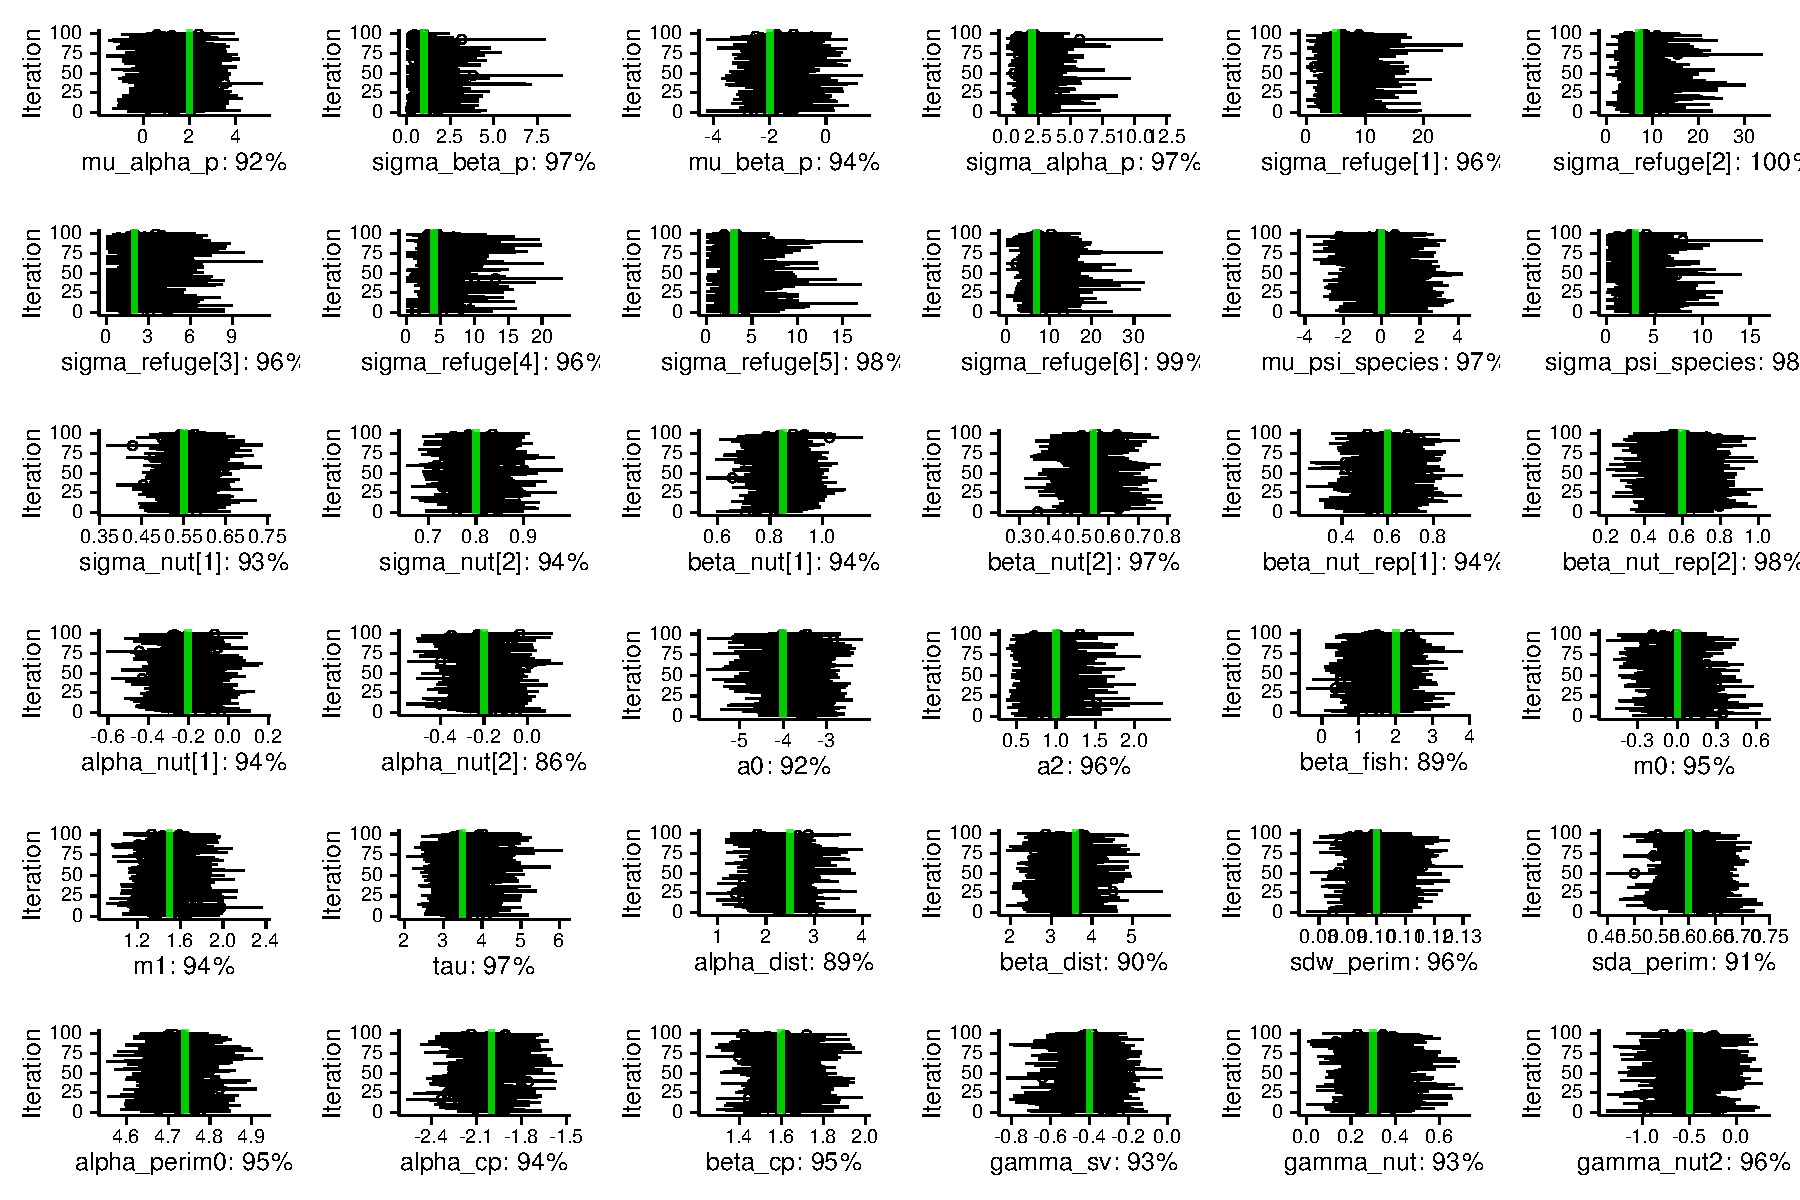
\includegraphics[width=150mm]{figs/ch3/fig_s1.pdf}
\label{3-a1}
\end{figure}

\begin{figure}[htbp]
\caption[Recovery of species-specific effects]{
Recovery of $\beta_\psi$ terms from the simulated 100 data sets. Red
indicates parameter estimates for which the HDI was entirely negative,
green indicates HDIs overlapping zero, and blue indicates HDIs that were
entirely positive.
}
\centering
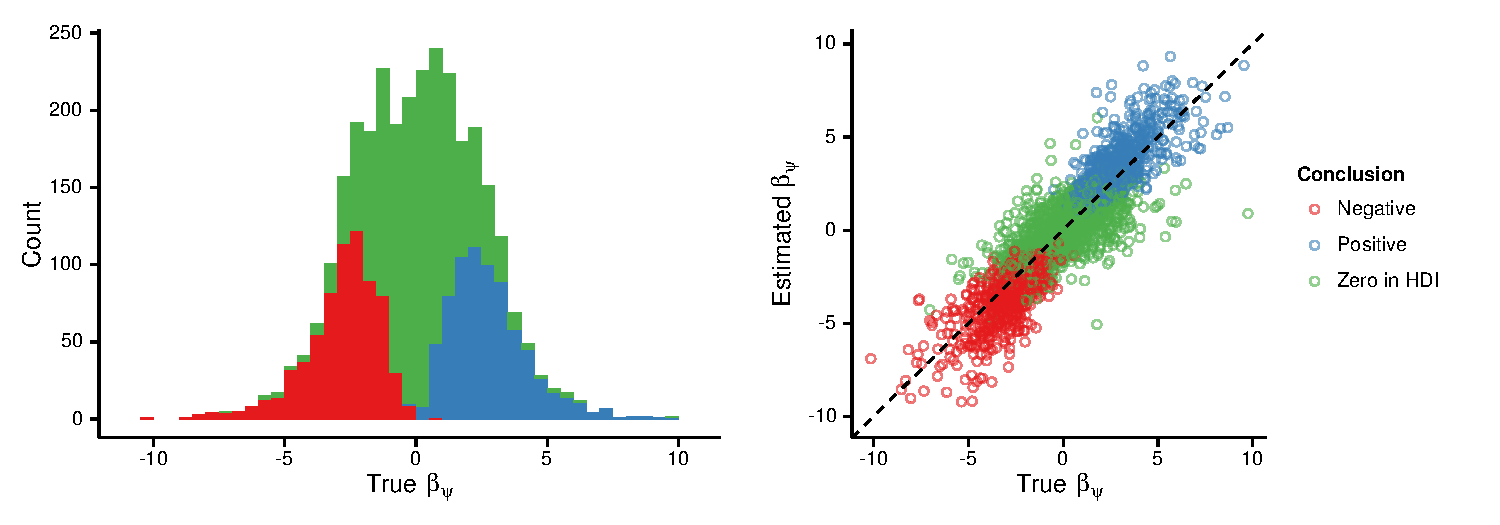
\includegraphics[width=150mm]{figs/ch3/fig_s2.pdf}
\label{3-a2}
\end{figure}

\begin{figure}[htbp]
\caption[Among refuge variance parameters for occupancy probabilities]{
Estimated among-refuge standard deviations in occupancy probabilities
for each species.
}
\centering
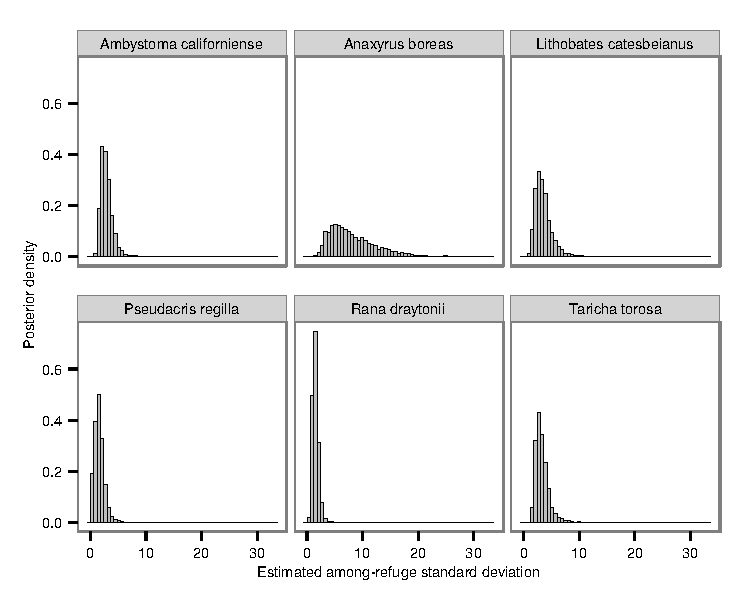
\includegraphics[width=150mm]{figs/ch3/fig_s3.pdf}
\label{3-a3}
\end{figure}

\begin{figure}[htbp]
\caption[Detection parameter estimates]{
Posterior estimates of detection probabilities for each species in early
and late summer. The interval represents the 95\% HDI, and the points
are placed at the posterior medians.
}
\centering
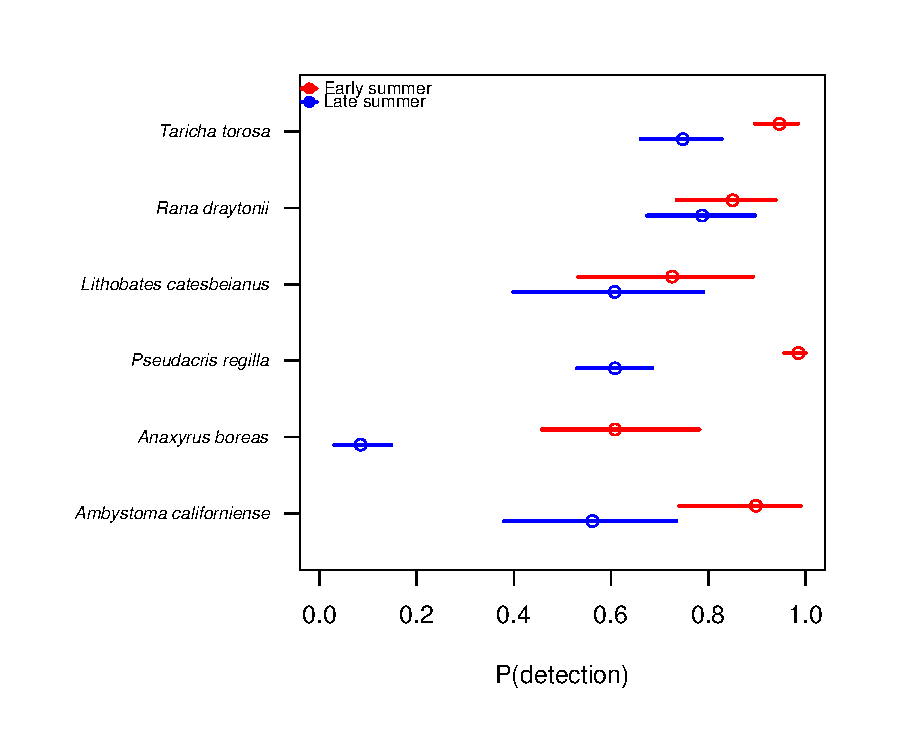
\includegraphics[width=150mm]{figs/ch3/fig_s4.pdf}
\label{3-a4}
\end{figure}

\begin{figure}[htbp]
\caption[Graphical independence checks]{
Graphical checks of independence assumptions implied by our model, used
to check for missing causal pathways.
}
\centering
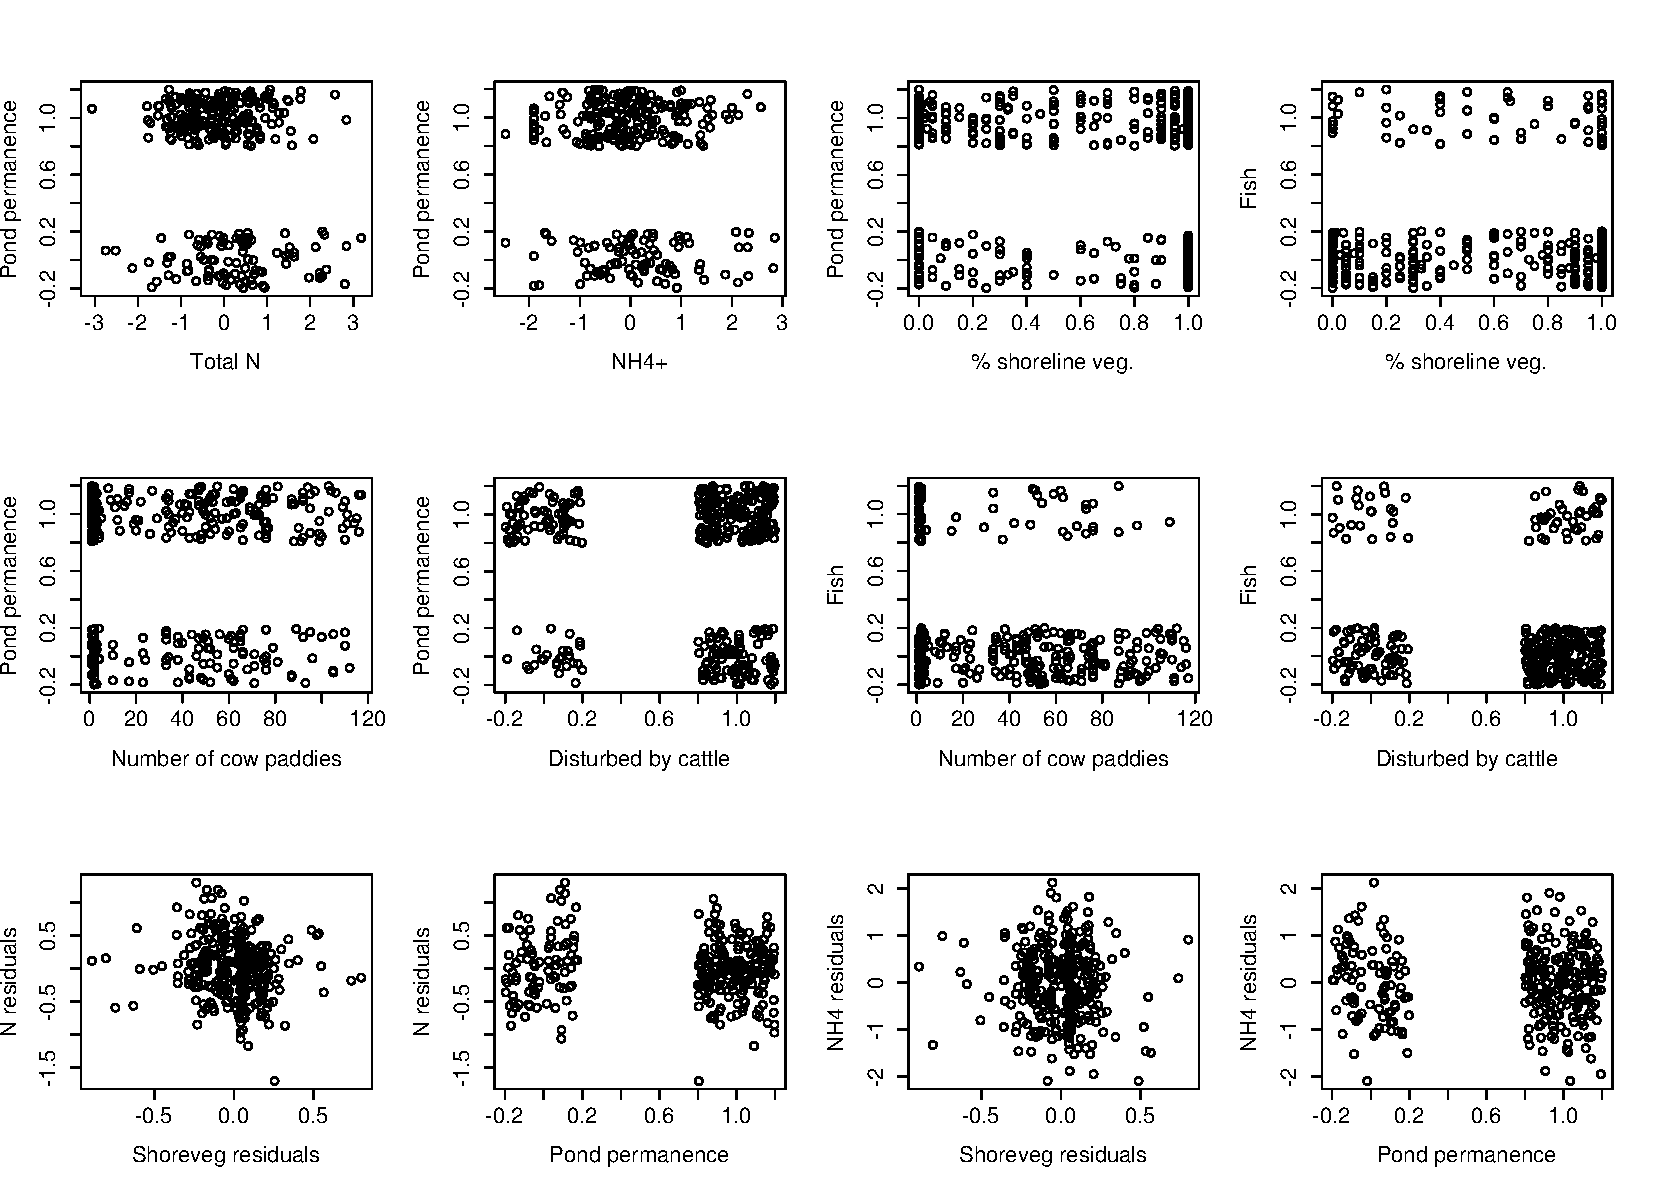
\includegraphics[width=150mm]{figs/ch3/fig_s5.pdf}
\label{3-a5}
\end{figure}
